\section{Problem Formulation and Benchmark}

\subsection{Defining a Tissue--MHC Prediction Context}

One prediction context corresponds to one tissue and one \plainMHCI{} restriction. For example, lung with HLA-A*02:01 and liver with the same allele are different contexts because the tissue differs. Let \(t\) denote a tissue and \(m\) an MHC-I restriction. We define the set of observed contexts as
\[
\mathcal{T}=\{\tau=(t,m)\}.
\]
Each benchmark row is represented by
\[
x_i=(p_i,\tau_i), \qquad y_i\in\{0,1\},
\]
where \(p_i\) is a nine-residue peptide and \(\tau_i\) identifies one tissue--MHC context. A positive label, \(y_i=1\), indicates positive ligand evidence in the target context. A comparison label, \(y_i=0\), indicates positive evidence under the same MHC restriction and parent protein in at least one other tissue, but no report in the target context. Thus, the pseudo-negative label represents absence of recorded evidence rather than experimentally verified non-presentation.

Given \((p,\tau)\), a model parameterized by \(\theta\) produces
\[
s_{\theta}(p,\tau)\in\mathbb{R},
\]
with larger values indicating stronger predicted evidence within tissue--MHC combination \(\tau\). Operationally, the model learns to rank a peptide reported in the target tissue above a comparison peptide matched by MHC restriction and parent protein. It is trained on individual peptide rows, while the paired construction controls example generation and evaluation. Because each tissue--MHC combination has its own prediction function, the benchmark evaluates previously represented combinations; it does not assess unseen tissues or unseen MHC restrictions.

\subsection{Pairing Peptides by Tissue, MHC Restriction, and Parent Protein}

Each pair \(j\) contains one positive peptide \(p_j^{+}\) and one pseudo-negative peptide \(p_j^{-}\) with evidence elsewhere but not in the target tissue. The two rows share the same target tissue, MHC restriction, and parent UniProt protein:
\[
t_j^{+}=t_j^{-}, \qquad
m_j^{+}=m_j^{-}, \qquad
u_j^{+}=u_j^{-}.
\]
This matching removes two easy explanations for a difference: the peptides cannot be separated merely because they use different \plainMHC{} molecules or come from different proteins. The remaining difference can include tissue-associated processing and presentation, but also differences in cell composition, study design, detection sensitivity, and annotation completeness. The benchmark therefore measures tissue-associated evidence, not a purified molecular mechanism.

We first calculate performance separately for every tissue--MHC combination and then give each combination equal weight, so common combinations do not dominate rare ones. We also report within-pair ordering accuracy:
\[
\begin{aligned}
    \operatorname{Acc}_{\mathrm{pair}}
&=
\frac{1}{N}\sum_{j=1}^{N}
\mathbf{1}\!\left[
s_{\theta}(p_j^{+},\tau_j)
>
s_{\theta}(p_j^{-},\tau_j)
\right].
\end{aligned}
\]
where \(N\) is the number of held-out pairs. This quantity is the fraction of pairs for which the peptide reported in the target tissue receives the higher score. AUROC measures ordering across all rows within a tissue--MHC combination, whereas within-pair accuracy directly evaluates the original MHC- and parent-matched comparison.

\subsection{Evidence Inclusion Criteria}

The human and mouse benchmarks are derived from the full ligand export of the \plainIEDB{} downloaded on July 4, 2026 \cite{vita2025iedb}. We apply the same biological inclusion rules to both species. We retain only clearly positive ligand records for \plainMHCI{} with an identifiable parent protein and a standard unmodified 9-amino-acid peptide:

\begin{itemize}
    \item a qualitative measurement whose normalized text begins with \emph{positive};
    \item a \plainMHCI{} restriction, with both peptide source and host matching Homo sapiens for the human benchmark or Mus musculus for the mouse benchmark;
    \item a human restriction matching the four-digit \plainHLA{} pattern \texttt{HLA-\ldots{}*dd:dd} (the extractor also accepts the equivalent colon-free four-digit form) or a restriction from the mouse major histocompatibility complex (\plainHtwo{}; written as \texttt{H2} in the processed identifiers) beginning with \texttt{H2-};
    \item a parent UniProt accession extracted from the molecule-parent web identifier (internationalized resource identifier; IRI) in the \plainIEDB{};
    \item a linear, unmodified peptide containing only the 20 standard amino acids;
    \item a peptide length of exactly nine residues; and
    \item deduplication before pairing by the exact peptide, restriction, tissue, and parent/source-protein annotation fields.
\end{itemize}

Source-tissue values are stripped of surrounding whitespace and retained as the exact names used in the \plainIEDB{}; distinct nonempty tissue strings are not merged after extraction. Empty or missing-value-like fields required to define a tissue--MHC combination are removed before benchmark filtering, excluding 857 otherwise eligible human pairs. Pair-consistency checks require both rows to have the same nonempty tissue and restriction. Retained \plainHLA{} and \plainHtwo{} strings are used directly as identifiers after the pattern checks above. Records without a parent UniProt accession are excluded because parent-protein matching is a defining control of the benchmark. Restricting the study to unmodified canonical 9-residue peptides for \plainMHCI{} provides a consistent sequence space, but excludes variable-length ligands, post-translationally modified peptides, and presentation by MHC-II.

\subsection{Constructing MHC- and Parent-matched Peptide Pairs}

For each target tissue--MHC combination, we compare a peptide reported in that tissue with another peptide from the same protein that is reported in a different tissue under the same MHC restriction. A fixed random state, 20260704, makes the following construction reproducible:

\begin{enumerate}
    \item Group all eligible ligand records by MHC restriction \(m\) and parent UniProt protein \(u\).
    \item For each target combination \((t,m,u)\), collect peptides with positive evidence in tissue \(t\).
    \item From other tissues represented in the same \((m,u)\) group, collect candidate comparison peptides with evidence elsewhere but not yet in the target tissue (pseudo-negative peptides).
    \item Exclude every candidate with a positive report in the target tissue--MHC combination \((t,m)\).
    \item Within each target combination and label, use each peptide at most once. For a given \((t,m,u)\) group, set the number of pairs to the smaller of the eligible positive and pseudo-negative counts and sample both sets without replacement.
    \item Randomly permute the selected pseudo-negatives and join them one-to-one with the selected positives.
    \item Assign a persistent pair identifier, preserve the reported-tissue and protein annotations, and verify that every identifier has exactly one row per label, identical tissue, restriction, and parent UniProt values in both rows, and no target-tissue report for the pseudo-negative.
\end{enumerate}

Every pair contributes one target-tissue peptide and one comparison peptide, so the dataset is deliberately balanced. This balance is useful for controlled ranking but does not resemble the natural frequency of presented peptides in a tissue sample. The reported scores therefore describe relative ranking within this constructed benchmark, not the probability that a peptide would be detected in a biological specimen.

\begin{figure*}[t]
\centering
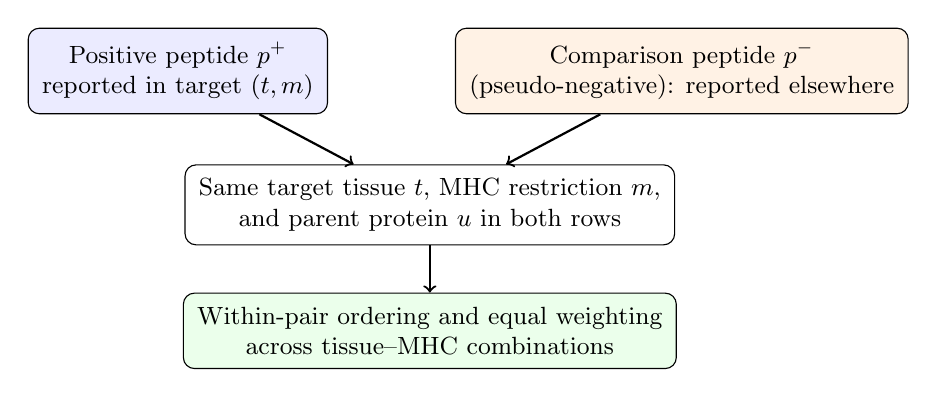
\begin{tikzpicture}[
    node distance=0.7cm,
    box/.style={draw,rounded corners,align=center,inner sep=5pt,font=\small},
    arr/.style={->,thick}
]
\node[box,fill=blue!8] (pos) at (-3.2,0) {Positive peptide \(p^{+}\)\\reported in target \((t,m)\)};
\node[box,fill=orange!10] (neg) at (3.2,0) {Comparison peptide \(p^{-}\)\\(pseudo-negative): reported elsewhere};
\node[box] (match) at (0,-1.7) {Same target tissue \(t\), MHC restriction \(m\),\\and parent protein \(u\) in both rows};
\node[box,fill=green!8] (eval) at (0,-3.3) {Within-pair ordering and equal weighting\\across tissue--MHC combinations};
\draw[arr] (pos) -- (match);
\draw[arr] (neg) -- (match);
\draw[arr] (match) -- (eval);
\end{tikzpicture}
\caption{Construction of a peptide pair matched by target tissue, MHC restriction, and parent protein. The comparison peptide has positive evidence elsewhere but no report in the target tissue--MHC context.}
\label{fig:pair-construction}
\end{figure*}

\subsection{Human Benchmark}

The human and mouse benchmarks use the same eligibility rule: a tissue--MHC combination is retained only when it contains more than 200 eligible MHC- and parent-matched peptide pairs. Under this rule, the human benchmark contains 157 tissue--HLA combinations, of which the smallest contains 201 pairs. Within each retained combination, 100 complete pairs are sampled without replacement for a saved internal test set, and all remaining pairs form the training partition. Random state 20260704 makes this division reproducible.

\begin{table}[tbp]
\centering
\caption{Human benchmark and saved internal test-set statistics.}
\label{tab:human-benchmark-stats}
\small
\begin{tabularx}{\columnwidth}{@{}>{\raggedright\arraybackslash}Xr@{}}
\toprule
Property & Value \\
\midrule
Tissue--HLA combinations & 157 \\
Tissues & 25 \\
\plainHLA{} alleles & 35 \\
Minimum eligible pairs per retained combination & 201 \\
Training pairs & 73,798 \\
Test pairs & 15,700 \\
Training rows & 147,596 \\
Test rows & 31,400 \\
Test pairs per combination & 100 \\
\bottomrule
\end{tabularx}
\end{table}

The 157 tissue--\plainHLA{} combinations summarized in Table~\ref{tab:human-benchmark-stats} form an incomplete and long-tailed tissue-by-HLA coverage matrix. Performance is therefore calculated separately for each combination before averaging with equal weight; pooling all rows would overemphasize combinations with more examples and could conceal weak performance in sparsely represented contexts. The saved internal test set excludes complete pair identifiers, but a peptide or parent protein may still occur in a different combination on both sides of the split. It therefore evaluates familiar tissue--HLA contexts rather than biological entities that are entirely absent from training.

For peptide-separated cross-validation, the complete 73,798-pair human training pool is considered jointly, while the separate 15,700-pair test set remains excluded. Pairs sharing either peptide are joined by following direct and indirect links before folds are formed. This produces 17,036 groups, including 10,923 containing multiple pairs; the largest contains 755 pairs. A reproducible assignment distributes complete groups across three folds while balancing the tissue--HLA combinations. Each held-out fold contains 24,598--24,600 pairs, each fitting set contains 49,198--49,200 pairs, all 157 combinations remain represented, and neither pair identifiers nor exact peptide sequences overlap between fitting and held-out data.

\subsection{Mouse Benchmark}

The mouse benchmark uses the same tissue-conditioned definition: the two peptides share their H2 restriction and parent protein, and a tissue--H2 combination is retained only when it contains more than 200 eligible pairs. This rule retains 24 tissue--H2 combinations; the smallest contains 224 pairs. Exactly 100 complete matched pairs per retained combination are sampled without replacement for the saved internal test set using random state 20260704, and the remainder form the training partition.

\begin{table}[tbp]
\centering
\caption{Mouse benchmark and saved internal test-set statistics.}
\label{tab:mouse-benchmark-stats}
\small
\begin{tabularx}{\columnwidth}{@{}>{\raggedright\arraybackslash}Xr@{}}
\toprule
Property & Value \\
\midrule
Tissue--H2 combinations & 24 \\
Tissues & 13 \\
\plainHtwo{} restrictions & 4 \\
Minimum eligible pairs per retained combination & 224 \\
Training pairs & 6,766 \\
Saved test pairs & 2,400 \\
Training rows & 13,532 \\
Saved test rows & 4,800 \\
\bottomrule
\end{tabularx}
\end{table}

The mouse inventory is summarized in Table~\ref{tab:mouse-benchmark-stats}. This saved internal partition was not examined until the model and analysis choices had been specified. A held-out peptide is absent from the training rows of the tissue--H2 combination being evaluated, but it may occur in training rows for another combination. Table~\ref{tab:mouse-fixed-overlap} makes this distinction explicit. For each test row, the audit first asks whether the same entity occurs in training for the current tissue--H2 combination and, only if it does not, whether it occurs in another combination. The three columns are therefore mutually exclusive.

\begin{table*}[t]
\centering
\caption{Mouse entity-overlap audit for the saved internal test set. Counts are test-row occurrences, except for pair identifiers, which are counted once per pair. ``Current combination'' means the tissue--H2 combination of the test row.}
\label{tab:mouse-fixed-overlap}
\footnotesize
\setlength{\tabcolsep}{3pt}
\begin{tabular}{@{}>{\raggedright\arraybackslash}p{2.8cm}
                    >{\centering\arraybackslash}p{2.4cm}
                    >{\centering\arraybackslash}p{2.4cm}
                    >{\centering\arraybackslash}p{2.4cm}@{}}
\toprule
Held-out entity (counted unit) & Current-combination training & Other-combination training only & Absent from all training \\
\midrule
Pair identifier (2,400 pairs) & 0 (0\%) & 0 (0\%) & 2,400 (100\%) \\
Peptide identity (4,800 rows) & 0 (0\%) & 4,047 (84.31\%) & 753 (15.69\%) \\
Parent UniProt (4,800 rows) & 710 (14.79\%) & 3,756 (78.25\%) & 334 (6.96\%) \\
\bottomrule
\end{tabular}
\end{table*}

Thus, a test peptide is new to the specific tissue--H2 combination being evaluated, even though most test rows contain a peptide already observed while fitting another combination. Among unique entities, 2,453 of 3,011 test peptides (81.47\%) and 967 of 1,088 parent proteins (88.88\%) occur somewhere in training. Parent proteins can also recur within the current combination because several matched pairs may come from the same protein. All 24 tissue--H2 combinations are represented in training. The saved test set is therefore an internal confirmation in familiar contexts with peptide reuse across contexts; it is not an evaluation of peptides, proteins, or biological combinations absent from all training, nor an independent external validation.

Mouse peptide-separated cross-validation applies the same transitive grouping of peptide-linked pairs to all 6,766 training-pool pairs. Complete groups are assigned to three folds while retaining all 24 tissue--H2 combinations in every held-out partition. Pair-identifier and exact-peptide overlap are both zero; the largest group contains 50 pairs, and each combination contributes 41--157 held-out pairs and 82--314 fitting pairs. These counts show that exact peptide separation across all combinations is feasible without deleting overlapping pairs after an initial random split.

\subsection{Evaluation Settings and Their Biological Meaning}

The evaluation design has three distinct layers: how observations are divided between fitting and evaluation, how independently trained models are combined, and how saved predictions are compared statistically. These layers do not define separate biological experiments. Table~\ref{tab:evaluation-protocols} distinguishes them in reader-facing language. In cross-validation, the training pool is divided into three parts and every part is predicted once by a model fitted on the other two. Independent training runs start the same model from different random states, whereas the random state used to reproduce pair sampling or fold assignment does not create another trained model. Model structure, tuning choices, training runs, and prediction averaging are specified before the relevant evaluation results are inspected.

\begin{table*}[t]
\centering
\caption{Evaluation settings and their relationships. A data setting changes which observations are available for fitting and evaluation. A model procedure changes how models are trained or combined without defining a new data split. A statistical comparison operates only on saved predictions.}
\label{tab:evaluation-protocols}
\fontsize{7.5}{8.5}\selectfont
\setlength{\tabcolsep}{1.5pt}
\begin{tabular}{@{}>{\raggedright\arraybackslash}p{2.25cm}
                    >{\raggedright\arraybackslash}p{1.6cm}
                    >{\raggedright\arraybackslash}p{3.75cm}
                    >{\raggedright\arraybackslash}p{3.75cm}@{}}
\toprule
Reader-facing setting & Layer & What is done & Purpose and relationship to the other settings \\
\midrule
Saved internal test set
& Data setting
& For each tissue--MHC combination, 100 complete positive--pseudo-negative pairs are kept outside the training file. A model fitted on all remaining rows scores this saved set once.
& Main internal benchmark for familiar tissue--MHC contexts. It contains different rows from both cross-validation analyses and is not an external cohort. \\
\midrule
Ordinary cross-validation with complete pairs kept together
& Data setting
& The training pool is divided into three folds within each tissue--MHC combination. Both rows from one pair always remain together; each row is predicted by a model fitted on the other two folds.
& Cross-validation used for model development and internal checking. The same peptide may still occur in fitting rows for another tissue--MHC combination. \\
\midrule
Ordinary cross-validation on the same pooled rows
& Comparison
& Complete pairs are kept together while exactly the same training-pool rows used by peptide-separated cross-validation are evaluated. Human results average three independent training runs and mouse results average five.
& Ordinary reference for the peptide-separated analysis. Both analyses score the same rows, but their fold memberships are not identical or matched pair by pair. \\
\midrule
Repeated training and prediction averaging on the saved test set
& Model descriptor plus saved test
& A previously chosen model is refitted on the full training file from each prespecified initialization; predictions on the saved test set are then averaged. The main mouse result uses five independent runs.
& Prespecification and prediction averaging describe model estimation, not a new type of data split. \\
\bottomrule
\end{tabular}
\end{table*}

\begin{table*}[t]
\ContinuedFloat
\centering
\caption[]{Guide to evaluation terms used in this study (continued).}
\fontsize{7.5}{8.5}\selectfont
\setlength{\tabcolsep}{1.5pt}
\begin{tabular}{@{}>{\raggedright\arraybackslash}p{2.25cm}
                    >{\raggedright\arraybackslash}p{1.6cm}
                    >{\raggedright\arraybackslash}p{3.75cm}
                    >{\raggedright\arraybackslash}p{3.75cm}@{}}
\toprule
Term used in the project & Layer & What is done & Purpose and relationship to other terms \\
\midrule
Peptide-separated cross-validation
& Data setting
& Pairs linked by any shared peptide sequence are placed in the same fold. A held-out peptide sequence is therefore absent from fitting rows for every tissue--MHC combination.
& Robustness test for new exact peptide identities in familiar tissue--MHC contexts. It does not require held-out tissues, MHC alleles, or parent proteins to be new. \\
\midrule
Prediction averaging under peptide-separated cross-validation
& Model procedure plus peptide-separated cross-validation
& The same peptide-separated folds are used for every independent training run, and the held-out predictions are averaged across runs.
& Repeated-model implementation of the preceding data setting; it is not an additional split. \\
\midrule
Transitive grouping of peptide-linked pairs
& Split algorithm
& Shared-peptide links are followed transitively: if pair A shares a peptide with B and B shares one with C, all three enter the same fold.
& The fold-building algorithm that enforces exact-peptide separation across all tissue--MHC combinations. It is not a separate biological setting. \\
\midrule
Within-combination comparison of ordinary and peptide-separated results
& Statistical analysis
& For each tissue--MHC combination, the ordinary result is compared with the peptide-separated result, and the resulting differences are summarized across combinations.
& Quantifies how sensitive performance is to the change in fold construction. Exact-peptide separation is not fully independent validation. \\
\bottomrule
\end{tabular}
\end{table*}

\begin{figure*}[t]
\centering
\begin{tikzpicture}[
    box/.style={draw,rounded corners,align=center,inner sep=5pt,font=\small},
    arr/.style={->,thick},
    note/.style={draw,rounded corners,align=center,inner sep=5pt,font=\small}
]
\node[box,text width=7.2cm] (input) at (0,0)
    {Matched peptide-pair benchmark\\
     {\scriptsize Same tissue, MHC restriction, and parent protein}};

% Saved internal test pathway.
\node[box,fill=blue!8,text width=5.1cm] (holdout) at (-4.4,-1.45)
    {Hold out 100 complete peptide pairs\\
     {\scriptsize from every tissue--MHC combination}};
\node[box,text width=5.1cm] (fit) at (-4.4,-3.10)
    {Fit the model on all remaining rows\\
     {\scriptsize Saved pairs are excluded from model fitting}};
\node[box,fill=blue!8,text width=5.1cm] (saved) at (-4.4,-4.85)
    {Saved internal test set\\
     {\scriptsize (fixed test)}\\
     {\scriptsize Internal evaluation in familiar contexts}};

% Cross-validation pathway.
\node[box,text width=7.4cm] (pool) at (3.5,-1.45)
    {Complete training pool\\
     {\scriptsize Saved internal test rows remain excluded}};
\node[box,fill=orange!10,text width=3.55cm] (pairfold) at (1.4,-2.80)
    {Keep both rows of each pair\\
     {\scriptsize together in one fold}};
\node[box,fill=green!8,text width=3.55cm] (peptidefold) at (5.6,-2.80)
    {Keep peptide-linked groups\\
     {\scriptsize together in one fold}};
\node[box,fill=orange!10,text width=3.55cm] (ordinary) at (1.4,-4.85)
    {Ordinary cross-validation\\
     {\scriptsize (standard OOF)}\\
     {\scriptsize A held-out peptide may occur in another fitting combination}};
\node[box,fill=green!8,text width=3.55cm] (separated) at (5.6,-4.85)
    {Peptide-separated cross-validation\\
     {\scriptsize (peptide-disjoint OOF)}\\
     {\scriptsize Every held-out peptide is absent from all fitting combinations}};

\node[box,text width=5.1cm] (descriptive) at (-4.4,-6.75)
    {Descriptive comparison only\\
     {\scriptsize The saved test set evaluates different rows}};
\node[box,fill=green!8,text width=7.4cm] (comparison) at (3.5,-6.75)
    {Compare ordinary and peptide-separated results\\
     {\scriptsize Within-combination sensitivity to excluding exact peptide identities}};
\node[note,text width=5.1cm] (estimation) at (-4.4,-8.20)
    {Independent training runs and prediction averaging\\
     {\scriptsize Model estimation, not an additional data split}};
\node[box,fill=green!8,text width=7.4cm] (question) at (3.5,-8.20)
    {Biological question: how much ranking signal remains\\
     for unseen exact peptide identities\\
     in familiar tissue--MHC contexts?};

\draw[arr] (input) -| (holdout);
\draw[arr] (input.east) -| ($(pool.north)+(1.0cm,0)$);
\draw[arr] (holdout) -- (fit);
\draw[arr] (fit) -- (saved);
\draw[arr] (pool) -- ++(0,-0.55) -| (pairfold);
\draw[arr] (pool) -- ++(0,-0.55) -| (peptidefold);
\draw[arr] (pairfold) -- (ordinary);
\draw[arr] (peptidefold) -- (separated);
\draw[arr,dashed] (saved) -- (descriptive);
\draw[arr] (ordinary.south) -- (ordinary.south |- comparison.north);
\draw[arr] (separated.south) -- (separated.south |- comparison.north);
\draw[arr] (comparison) -- (question);
\end{tikzpicture}
\caption{Relationship among the evaluation settings. The saved-test pathway evaluates
different rows after fitting on the complete remaining training set. The two
cross-validation pathways evaluate the same pooled rows but differ in what is kept
together when folds are formed: complete pairs in the ordinary analysis, or entire
groups connected by a shared peptide in the peptide-separated analysis. Repeated
training runs and prediction averaging describe model estimation rather than a new
data split. Only the two cross-validation results support a within-combination
sensitivity comparison.}
\label{fig:evaluation-setting-relationships}
\end{figure*}

\paragraph{What is actually predicted.}
The benchmark is constructed from matched peptide pairs, but the main neural models do not receive two peptides simultaneously. They score one peptide row at a time using its sequence and tissue--MHC identity. Pair identifiers are used to create balanced recorded-positive and pseudo-negative examples and to keep the two rows of a pair in the same data partition. Training applies a separate present/absent loss to each row, and AUROC and AUPRC compare all positive and pseudo-negative rows within a tissue--MHC combination. Within-pair ordering accuracy asks the complementary question of whether the recorded-positive peptide receives the higher score. Keeping both members of a pair together protects data integrity; it does not turn the main training objective into a direct two-peptide ranking loss.

\paragraph{Saved internal test set.}
For each tissue--MHC combination, the dataset builder randomly selects 100 complete pairs for the test file and assigns the remaining pairs to the training file. Because a peptide is used at most once within a combination during pair construction, a test peptide is absent from training rows for that same combination. The sequence may nevertheless occur in another fitting combination and can then influence shared model parameters. This test set therefore measures internal discrimination in already represented biological contexts while allowing information sharing across combinations. Saving the partition and analysis choices before evaluation does not imply that the test set has never influenced the wider research process. The human test set was examined repeatedly during long-term model development; the mouse test set was opened only after the model, training runs, and prediction-averaging rule had been specified.

\paragraph{Ordinary cross-validation with complete pairs kept together.}
This analysis uses only the training file. Within each tissue--MHC combination, complete pairs are distributed across three nearly equal folds. Two folds fit the model and the third is held out; rotating this role gives one prediction for every row in the pool. The model predicting a row has therefore fitted neither member of its pair. The construction rule also prevents exact peptide reuse within that tissue--MHC combination, but the peptide may still appear in a different fitting combination. This is a development-stage estimate for familiar biological contexts, not an independent validation dataset. It also differs from the saved test set in both the evaluated rows and the amount of fitting data, so the two numerical results can only be compared descriptively.

\paragraph{Ordinary cross-validation on the same pooled rows.}
For the direct sensitivity analysis, ordinary cross-validation is repeated on exactly the same training-pool rows as the peptide-separated analysis. The model family, independent training runs, number of folds, and pooled evaluation rows are the same, and fold sizes are closely matched within each tissue--MHC combination. Fold membership is nevertheless constructed independently: corresponding folds are not forced to contain the same pairs, proteins, or peptide-linked groups. The comparison is informative because both analyses calculate each metric from the same labeled rows for a given biological combination. It measures sensitivity to alternative training-data partitions rather than isolating a causal contribution from repeated peptide identities.

\paragraph{Cross-validation with held-out peptides absent from all fitting combinations.}
To remove exact peptide reuse across combinations, each peptide pair is represented as a point in a network. Two points are linked when either pair contains the same peptide sequence. Pairs connected directly or through intermediate links form one group, and that complete group is assigned to one fold. Consequently, neither member of a held-out pair nor any exact copy of those sequences in another combination can occur in the fitting rows. All tissue--MHC combinations remain represented during fitting. The analysis therefore asks whether the model can recognize tissue-associated sequence preferences for peptide identities it has not previously seen while operating in familiar tissue and MHC contexts.

This construction changes more than the presence of an exact duplicate. A shared peptide can connect a chain of otherwise different pairs, causing the entire chain to move together. The resulting folds can also differ in parent-protein composition and in the distribution of related sequence patterns. Table~\ref{tab:oof-overlap-audit} illustrates this point: although parent protein is not an input to the main models and is not explicitly separated, its overlap decreases markedly when peptide-linked groups are kept intact. The performance difference is therefore best interpreted as sensitivity to separating exact peptide identities. It does not isolate a pure or mechanism-specific contribution from repeated peptides.

\begin{table*}[t]
\centering
\caption{Entity overlap in the two cross-validation analyses using the same pooled rows. Pair overlap is the number of complete pair identifiers shared between fitting and held-out rows. Peptide values give the fold range for the percentage of unique held-out peptide sequences also present in fitting. Protein values give the three-fold mean percentage of unique held-out parent proteins present in fitting.}
\label{tab:oof-overlap-audit}
\fontsize{7.5}{8.5}\selectfont
\setlength{\tabcolsep}{3pt}
\begin{tabularx}{\textwidth}{@{}>{\raggedright\arraybackslash}p{0.9cm}
                                  >{\raggedright\arraybackslash}X
                                  >{\centering\arraybackslash}p{1.45cm}
                                  >{\centering\arraybackslash}p{1.8cm}
                                  >{\centering\arraybackslash}p{1.8cm}@{}}
\toprule
Species & Cross-validation setting & Pair overlap & Peptide overlap & Protein overlap \\
\midrule
Human & Ordinary cross-validation & 0 & 69.19--69.91\% & 90.64\% \\
Human & Peptide-separated cross-validation & 0 & 0\% & 65.26\% \\
\midrule
Mouse & Ordinary cross-validation & 0 & 71.43--72.12\% & 80.69\% \\
Mouse & Peptide-separated cross-validation & 0 & 0\% & 14.37\% \\
\bottomrule
\end{tabularx}
\end{table*}

\paragraph{Prespecified models, cohort-relative score combination, and statistical comparison.}
The human model structure and the mouse comparison families, training budgets, independent initializations, and prediction-averaging rules were specified before the peptide-separated results were examined. This prevents direct tuning to those results, but it does not make the experiment fully nested: the model structures had already been developed using ordinary cross-validation predictions from the same training-pool rows. The peptide-separated analysis is therefore a robustness evaluation of previously developed model families. In addition, the human model converts the two pathway outputs to relative order positions among peptides in each held-out tissue--MHC combination before averaging them. This transformation uses no held-out labels, but the final score is relative to the other peptides evaluated in that cohort rather than a stand-alone calibrated probability. Mouse neural controls instead average probabilities across independent training runs.

The paired statistics are calculated after prediction and do not create another split. Ordinary and peptide-separated results are compared separately within each tissue--MHC combination because both analyses cover the same pooled evaluation rows. This correspondence reduces variation caused by evaluating different sets of biological combinations, but it does not remove variation arising from fold membership, peptide-linked group structure, or the resulting composition of the fitting data.

\paragraph{Scope of the biological conclusion.}
The ordinary evaluation asks whether peptide sequence helps distinguish recorded positives from matched pseudo-negatives in familiar tissue--MHC contexts while information may be shared across combinations. The peptide-separated evaluation asks whether a substantial part of that signal remains when the exact held-out sequences are removed from all fitting combinations. Neither analysis demonstrates that a pseudo-negative is biologically never presented, identifies a causal antigen-processing mechanism, or evaluates a new tissue, MHC allele, tissue--MHC combination, parent protein, study, or external cohort. Parent proteins, studies, experimental platforms, and related peptide motifs may still recur. The peptide-separated result is therefore an internal robustness analysis rather than fully independent biological validation.
